\documentclass[9pt]{beamer}
\mode<presentation>

% Theme choice:
\usetheme{Madrid}%Darmstadt 
\usepackage{xcolor}
\definecolor{mGreen}{rgb}{0,0.6,0}
\definecolor{mRed}{rgb}{0.6,0,0}
\usecolortheme[RGB={0,100,50}]{structure}
 \usefonttheme{structurebold} 
\setbeamercovered{invisible}
%\setbeamertemplate{navigation symbols}{}
\usepackage{dynblocks}
\usepackage{textpos}
\usepackage{amsfonts}
\usepackage{amsmath}
\usepackage{amssymb}
\usepackage{amsthm}
\usepackage{listings}
\usepackage{tikz}
\usepackage{pgfplots}
\pgfplotsset{compat=1.18}
\newtheorem{teorema}{Teorema}\usepackage{mathtools}
\renewcommand{\proofname}{Prova}
\usepackage[portuguese]{babel}

\uselanguage{Portuguese}
\languagepath{Portuguese}

\deftranslation[to=Portuguese]{Theorem}{Teorema}
\deftranslation[to=Portuguese]{Lemma}{Lema}
\deftranslation[to=Portuguese]{Corollary}{Corolário}
\deftranslation[to=Portuguese]{Proof}{Prova}

\usepackage{dutchcal}
\usepackage{hyperref}
\usepackage[utf8]{inputenc}
\usepackage[T1]{fontenc}
\usepackage{amsthm}


\usepackage[affil-it]{authblk} 
\usepackage{etoolbox}
\usepackage{lmodern}

\makeatletter
\patchcmd{\@maketitle}{\LARGE \@title}{\fontsize{18}{19.2}\selectfont\@title}{}{}
\makeatother

\renewcommand\Authfont{\fontsize{12}{14.4}\selectfont}
\renewcommand\Affilfont{\fontsize{9}{10.8}\itshape}

% Title page details: 
\title[Presentation]{ENGENHARIA DA QUALIDADE E CONFIABILIDADE} %add title


\institute[UniRV]{\textbf{\large  \textcolor{structure}{\textbf{\large
Aprofundando nos Conceitos de Confiabilidade segundo Sommerville.
}} %add name 
% \hspace{0.5pt}
\\ \qquad
\\Professor: Me. Sergio Souza Novak 
\\Faculdade de Engenharia de Software}
} 
% \titlegraphic{\includegraphics[width=5cm]{msu.eps}}
\titlegraphic{
\includegraphics[width=5cm]{Universidade_de_Rio_Verde.jpg}}
\date{}

% Logo only on title page
%\logo{
\includegraphics[width=1cm,keepaspectratio]{Logo.png}}
\usepackage[pscoord]{eso-pic}


\begin{document}

% Title page frame
%\begin{frame}
    %\titlepage 
%\end{frame}
\frame[plain]{\titlepage}
%logo
\AddToShipoutPictureFG{
    \put(\LenToUnit{.92\paperwidth},
    \LenToUnit{.185\paperheight})
    {\vtop{{\null}
    \makebox{
\includegraphics[width=.8cm,keepaspectratio]{Universidade_de_Rio_Verde.jpg}}}}}


\begin{frame}{Sumário}
  \tableofcontents
\end{frame}
\section{Disponibilidade de serviços e desafios}
% Slide 1: Introdução a Fermat
\begin{frame}{Disponibilidade de serviços e desafios}

\small

\textbf{Dependência do Software}

A forte dependência de sistemas de software em praticamente todos os aspectos
da vida profissional e pessoal implica que:

\begin{itemize}
    \item Esperamos que o software esteja disponível quando necessário;
    \item Funcione no início da manhã, à noite, nos finais de semana e feriados;
    \item Opere continuamente (24h por dia, 7 dias por semana);
    \item Preserve dados e informações pessoais;
    \item Execute suas funções sem falhas ou interrupções.
\end{itemize}

\vspace{0.3cm}
\end{frame} 
\begin{frame}{Disponibilidade de serviços e desafios}

\textbf{Evolução da Confiabilidade}

O avanço de: 
\begin{itemize}
    \item Técnicas de Engenharia de Software;
    \item Linguagens de programação mais robustas;
    \item Processos eficazes de garantia da qualidade;
\end{itemize}

resultou em melhorias significativas na confiabilidade nas últimas décadas.

\vspace{0.3cm} 

\begin{block}{Desafios Atuais}

Apesar dos avanços:
\begin{itemize}
    \item Falhas de sistema ainda ocorrem;
    \item A disponibilidade pode ser comprometida;
    \item Resultados incorretos podem ser produzidos.
\end{itemize}
\end{block}

\end{frame} 
\section{Problemas possíveis}  

% Slide 1: Erro Humano
\begin{frame}{1. Erro Humano (Engano)}
      \begin{figure}[h] % [h] tenta posicionar "aqui" (here)
    \centering % Centraliza a imagem
    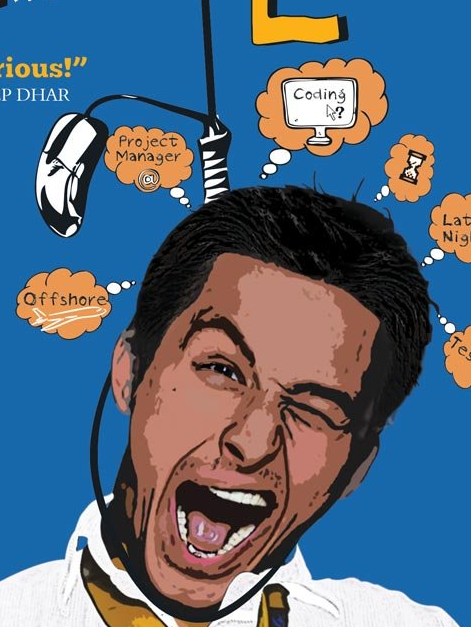
\includegraphics[width=0.2\linewidth]{loser_programmer.png}
    % \caption{falha}
\end{figure}
  \begin{block}{Definição}
    Comportamento ou ação humana que resulta na introdução de defeitos em um sistema.
  \end{block}
  
  \vspace{0.5cm}
  \textbf{Exemplo nas Estações Meteorológicas:}
  \begin{itemize}
    \item O programador estabelece a lógica: $T_{transmissão} = T_{atual} + 1h$.
    \item \textbf{A Falha de Raciocínio:} O desenvolvedor não considera a transição de ciclo do relógio de 24 horas.
    \item Ocorre no nível cognitivo do desenvolvedor.
  \end{itemize}
\end{frame}

% Slide 2: Defeito de Sistema
\begin{frame}[fragile]{2. Defeito de Sistema (Bug)}
  \begin{block}{Definição}
    Uma característica física ou lógica no software que pode levar a um erro de sistema quando executada.
  \end{block}

  \textbf{Representação em Java:}
  \begin{lstlisting}
public class EstacaoMeteorologica {
    private int horarioTransmissao;

    public void agendarProxima(int horarioAtual) {
        // O DEFEITO: Falta logica para resetar o dia (24h)
        this.horarioTransmissao = horarioAtual + 1; 
        
        // Se horarioAtual for 23, o estado interno
        // passara a ser 24 (Estado de Erro).
    }
}
  \end{lstlisting}

  \begin{itemize}
    \item O defeito reside na \textbf{ausência} de uma condicional que trate o limite: $\texttt{if (novoHorario >= 24) ...}$
  \end{itemize}
\end{frame}

% Slide 3: Erro de Sistema
\begin{frame}{3. Erro de Sistema (Estado Errôneo)}
  \begin{block}{Definição}
    Um estado interno incorreto do sistema durante sua execução, resultante de um defeito.
  \end{block}
  
  \vspace{0.5cm}
  \begin{figure}[h] % [h] tenta posicionar "aqui" (here)
    \centering % Centraliza a imagem
    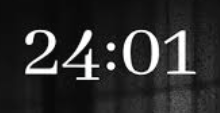
\includegraphics[width=0.2\linewidth]{24e1.png}
    \caption{Estado de erro no sistema}
\end{figure}
  \textbf{Manifestação em Tempo de Execução:}
  \begin{itemize}
    \item O código defeituoso é executado quando o relógio marca 23h30.
    \item O valor da variável \texttt{horarioDeTransmissao} torna-se \textbf{24h30}.
    \item No sistema de 24h, o valor correto deveria ser \textbf{00h30}.
    \item O sistema ainda não "travou", mas seu estado interno está corrompido.
  \end{itemize}
\end{frame}
 
% Slide 4: Falha de Sistema
\begin{frame}{4. Falha de Sistema}
  \begin{block}{Definição}
    Um evento em que o sistema não presta o serviço esperado pelo usuário final.
  \end{block}
    \begin{figure}[h] % [h] tenta posicionar "aqui" (here)
    \centering % Centraliza a imagem
    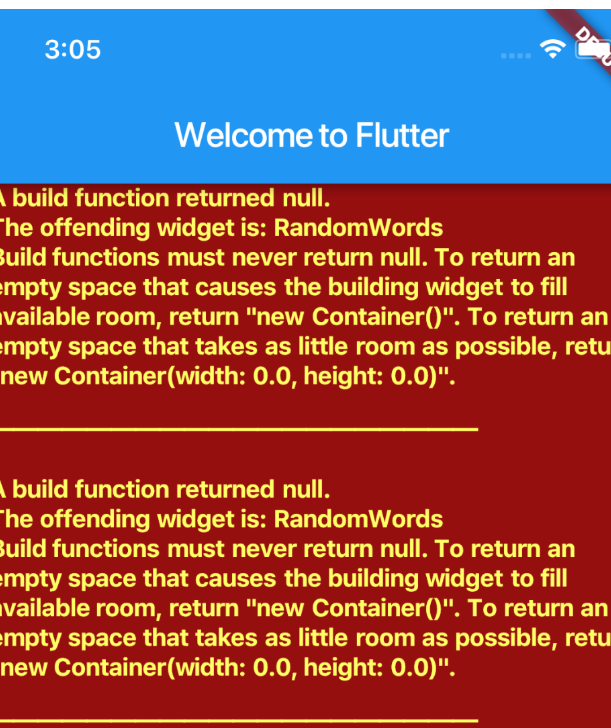
\includegraphics[width=0.5\linewidth]{falha.png}
    \caption{falha}
\end{figure}
 
\end{frame}
% Slide 4: Falha de Sistema
\begin{frame}{4. Falha de Sistema}
 
    \begin{figure}[h] % [h] tenta posicionar "aqui" (here)
    \centering % Centraliza a imagem
    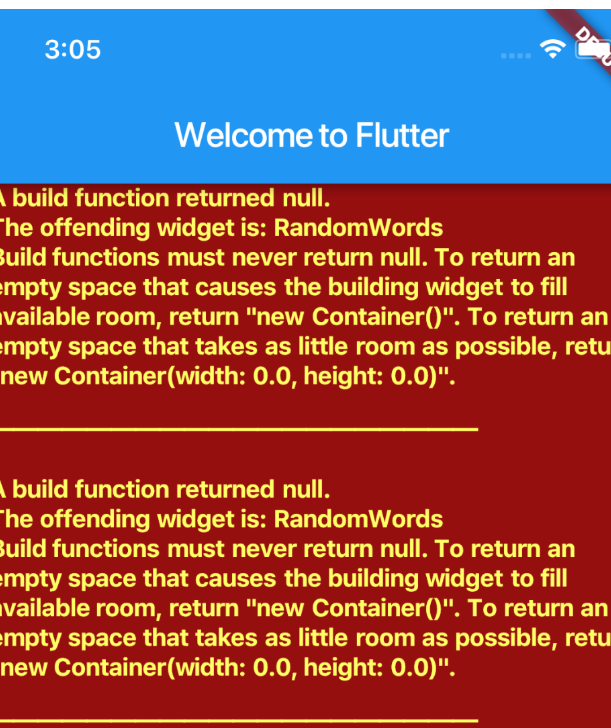
\includegraphics[width=0.2\linewidth]{falha.png}
    \caption{falha}
\end{figure}
  \vspace{0.5cm}
  \textbf{O Impacto Final:}
  \begin{itemize}
    \item O escalonador de tarefas busca por um horário válido para transmitir.
    \item Como \textbf{24h30} é um horário inexistente/inválido para o protocolo, a transmissão não ocorre.
    \item \textbf{Resultado:} Perda de dados e interrupção do serviço meteorológico.
  \end{itemize}
\end{frame}

\section{Ponderações sobre os Problemas nos Sistemas}  


\begin{frame}{Os defeitos de sistema não resultam necessariamente em erros, que por sua vez não resultam necessariamente em falhas de sistema}
\centering
\vspace{1cm}

\Large
\textbf{Defeitos $\not\Rightarrow$ Erros $\not\Rightarrow$ Falhas}

\vspace{0.5cm}

\small
Um sistema pode conter defeitos que nunca se manifestam como erros durante a execução.  
Da mesma forma, erros podem ocorrer sem causar falhas visíveis para os usuários.
\end{frame}







% Slide 1: Código não executado
\begin{frame}[fragile]{1. O Defeito pode nunca ser executado}
  \begin{itemize}
    \item Um \textbf{defeito} (bug no código) só se torna um \textbf{erro} (estado inválido) se a linha de código específica for processada.
    \item Dependendo do uso do software, certas funções ou ramos condicionais (\textit{if/else}) podem nunca ser ativados.
  \end{itemize}

  \begin{block}{Exemplo: Variável não inicializada}
    \begin{lstlisting}[language=Java, basicstyle=\ttfamily\small]
public void processarDados(boolean condicaoRara) {
    int valor; // Defeito: Nao inicializada
    if (condicaoRara) {
        System.out.println(valor + 10); // Erro ocorre aqui
    }
}
    \end{lstlisting}
  \end{block}
  
  \textbf{Resultado:} Se \texttt{condicaoRara} for sempre \texttt{false}, o defeito permanece latente e o sistema nunca entra em estado de erro.
\end{frame}

% Slide 2: Erros Transitórios
\begin{frame}{2. Erros Transitórios}
  \begin{itemize}
    \item Um \textbf{erro} (estado interno incorreto) pode existir temporariamente na memória, mas ser "atropelado" antes de causar uma \textbf{falha} visível.
    \item O estado é reiniciado por uma nova entrada ou processamento subsequente.
  \end{itemize}

  \begin{exampleblock}{Cenário de Sobreposição}
    \begin{enumerate}
        \item O sistema calcula um horário de transmissão inválido: \texttt{24h15} (\textbf{Estado de Erro}).
        \item Antes do horário de transmissão chegar, o operador altera manualmente a configuração ou o sistema recebe um \textit{reset} de sincronização.
        \item O valor é atualizado para \texttt{00h20} (\textbf{Estado Válido}).
    \end{enumerate}
  \end{exampleblock}
  
  \textbf{Conclusão:} O erro existiu, mas foi efêmero e não gerou impacto externo.
\end{frame}

% Slide 3: Proteção e Detecção
\begin{frame}{3. Mecanismos de Tolerância a Falhas}
  \begin{itemize}
    \item Sistemas robustos são projetados para prever que erros ocorrerão.
    \item Mecanismos de \textbf{detecção} e \textbf{recuperação} impedem que o estado de erro se transforme em uma falha de serviço.
  \end{itemize}



  \begin{block}{Estratégias Comuns}
    \begin{itemize}
        \item \textbf{Validação de Dados:} O sistema checa se o valor é plausível antes de usá-lo.
        \item \textbf{Redundância:} Outro módulo calcula o mesmo dado e compara os resultados.
        \item \textbf{Exceções:} O erro é capturado (\texttt{try-catch}) e tratado graciosamente.
    \end{itemize}
  \end{block}
\end{frame}

\begin{frame}{Corrigir defeitos em recursos não utilizados não afeta a confiabilidade do sistema}
\centering
\vspace{0.5cm}

\Large

\vspace{0.5cm}

\small
A distinção entre \textbf{defeitos, erros e falhas} leva a três abordagens complementares utilizadas para melhorar a confiabilidade de um sistema:
\vspace{0.5cm}

\begin{itemize}
    \item Identificação e correção de defeitos críticos;
    \item Prevenção de erros durante a execução;
    \item Minimização do impacto de falhas no serviço prestado.
\end{itemize}

\end{frame}
% Slide 1: Prevenção de Defeitos
\begin{frame}{1. Prevenção de Defeitos}
  \begin{block}{Objetivo}
    Utilizar abordagens de projeto e implementação que evitem a introdução de erros humanos no código, minimizando defeitos desde a origem.
  \end{block}

  \textbf{Técnicas e Abordagens:}
  \begin{itemize}
    \item \textbf{Linguagens Fortemente Tipadas:} Permitem que o compilador detecte inconsistências antes da execução (ex: Java, Rust).
    \item \textbf{Evitar Construtos Propensos a Erros:} Minimizar o uso de ponteiros ou manipulação direta de memória.
    \item \textbf{Padrões de Projeto:} Uso de boas práticas de arquitetura para reduzir a complexidade.
  \end{itemize}
  
  \textit{"Menos defeitos introduzidos significam menos chances de falhas operacionais."}
\end{frame}

% --- O SLIDE COM CÓDIGO AMPLIADO ---
\begin{frame}[fragile]{Comparativo de Confiabilidade: C vs. Java}
    \begin{columns}[T] % [T] alinha as colunas pelo topo
        % Coluna C
        \begin{column}{0.48\textwidth}
            \textbf{\textcolor{mRed}{Linguagem C}}
            \begin{itemize}
                \item Gestão Manual.
                \item Ponteiros Diretos.
                \item Verificação Fraca.
            \end{itemize}
            \begin{lstlisting}[language=C, basicstyle=\ttfamily\small, xleftmargin=-5pt]
int arr[5];
arr[10] = 100; 
// Defeito! 
// Acesso invalido.
            \end{lstlisting}
        \end{column}

        % Coluna Java
        \begin{column}{0.48\textwidth}
            \textbf{\textcolor{mGreen}{Java}}
            \begin{itemize}
                \item Gestão Automática.
                \item Sem Ponteiros.
                \item Verificação Forte.
            \end{itemize}
            \begin{lstlisting}[language=Java, basicstyle=\ttfamily\small, xleftmargin=-5pt]
int[] arr = new int[5];
arr[10] = 100; 
// Excecao!
// Erro detectado.
            \end{lstlisting}
        \end{column}
    \end{columns}

    \vspace{0.3cm} 
    \begin{block}{Conclusão}
        O Java interrompe o erro antes que ele vire uma falha catastrófica, enquanto o C permite a execução em estado corrompido.
    \end{block}
\end{frame} 
% Slide 2: Detecção e Correção de Defeitos
\begin{frame}{2. Detecção e Correção de Defeitos}
  \begin{block}{Objetivo}
    Descobrir e remover defeitos remanescentes através de Verificação e Validação (V\&V) antes da implantação do sistema.
  \end{block}



% [Image of V-model software development life cycle showing verification and validation stages]


  \textbf{Estratégias Principais:}
  \begin{itemize}
    \item \textbf{Análise Estática:} Revisão de código e ferramentas que buscam padrões de erro sem executar o programa.
    \item \textbf{Teste Sistemático:} Execução de casos de teste para garantir que o software atenda aos requisitos.
    \item \textbf{Depuração (Debugging):} Localização e correção da causa raiz dos defeitos encontrados.
    \item \textbf{Importância:} Fundamental para convencer \textit{stakeholders} e órgãos reguladores sobre a dependabilidade do sistema.
  \end{itemize}
\end{frame}


\begin{frame}{1. Erro Humano (Engano)}
      \begin{figure}[h] % [h] tenta posicionar "aqui" (here)
    \centering % Centraliza a imagem
    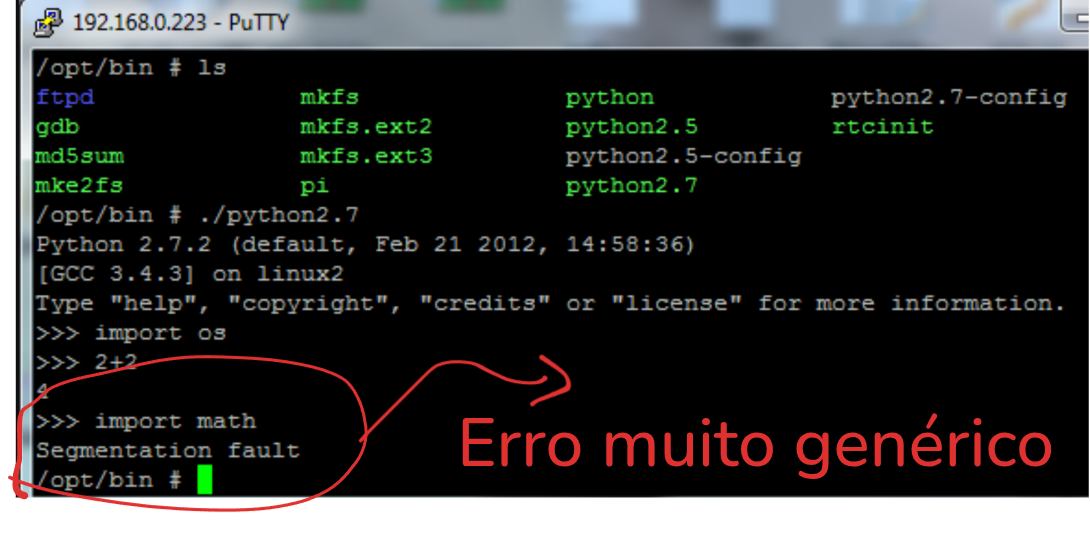
\includegraphics[width=\linewidth]{segmentation_fault.png}
    % \caption{falha}
\end{figure}
\end{frame}


% Slide 3: Tolerância a Defeitos
\begin{frame}{3. Tolerância a Defeitos}
  \begin{block}{Objetivo}
    Garantir que, mesmo na presença de defeitos ou estados inesperados, o sistema consiga se recuperar e evitar uma falha total.
  \end{block}



  \textbf{Níveis de Implementação:}
  \begin{itemize}
    \item \textbf{Abordagens Simples:} Verificações em tempo de execução (\textit{runtime checks}) e tratamento de exceções.
    \item \textbf{Sistemas Críticos:} Uso de redundância de hardware e software (Arquiteturas Tolerantes a Falhas).
    \item \textbf{Gerenciamento de Erros:} Detecção de estados inválidos e retorno a um estado seguro conhecido.
  \end{itemize}
  
  \textit{Essencial quando são necessários níveis altíssimos de disponibilidade e confiabilidade.}
\end{frame}


\section{Custo de Detecção vs. Erros Residuais}  

% --- SLIDE COM O GRÁFICO DE CUSTO ---
\begin{frame}{Custo de Detecção vs. Erros Residuais}
    \begin{columns}
        % Coluna da Imagem
        \begin{column}{0.9\textwidth}
            \begin{figure}
                \centering
                % Verifique se o nome do arquivo no seu painel lateral 
                % e exatamente este. Caso mude o nome no upload, mude aqui.
                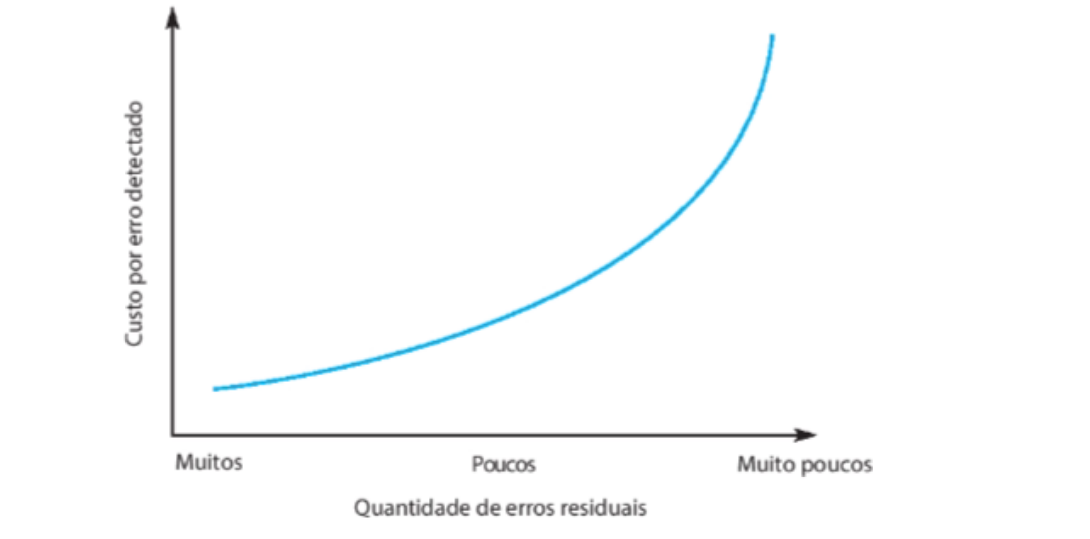
\includegraphics[width=\textwidth]{grafico1.png}
            \end{figure}
        \end{column}

    \end{columns}
    
        % Coluna de Texto
            \begin{block}{Análise da Curva}
                \begin{itemize}
                    \item \textbf{Custo Exponencial:} Remover os últimos erros é drasticamente mais caro.
                    \item \textbf{Decisão de Projeto:} Onde parar a detecção depende da criticidade do sistema.
                \end{itemize}
            \end{block}
    \small{Sistemas de altíssima disponibilidade operam na extremidade direita da curva.}
\end{frame}

% --- SLIDE: O DILEMA ECONÔMICO DA CONFIABILIDADE ---
\begin{frame}{O Dilema Econômico da Confiabilidade}
    \begin{itemize}
        \item \textbf{Custo Exponencial:} O esforço para encontrar e remover defeitos remanescentes aumenta drasticamente conforme o sistema se torna mais confiável.
        \item \textbf{Ponto de Retorno Decrescente:} Gasta-se cada vez mais tempo e esforço para encontrar cada vez menos defeitos, tornando o processo injustificável em certo ponto.
    \end{itemize}

    \begin{columns}[T]
        \begin{column}{0.5\textwidth}
            \begin{block}{Justificativa Econômica}
                \small
                As empresas aceitam \textbf{defeitos residuais} porque o custo da falha pode ser menor que o custo de remoção pré-entrega.
            \end{block}
        \end{column}
        \begin{column}{0.45\textwidth}
            \begin{block}{Níveis de Tolerância}
                \small
                \begin{itemize}
                    \item \textbf{Produtos de prateleira:} Nível de defeitos relativamente alto.
                    \item \textbf{Sistemas críticos:} Nível de defeitos bem mais baixo.
                \end{itemize}
            \end{block}
        \end{column}
    \end{columns}

    \vspace{0.3cm}
    \begin{alertblock}{Além da Economia}
        A decisão de lançar um software não é apenas financeira; deve-se considerar a \textbf{aceitabilidade social e política} de uma possível falha.
    \end{alertblock}
\end{frame}
\section{Diferenças entre Confiabilidade e Disponibilidade}  

% --- SLIDE: DEFINIÇÕES FORMAIS ---
\begin{frame}{Confiabilidade vs. Disponibilidade}
    \begin{block}{1. Confiabilidade (Reliability)}
        A probabilidade de operação \textbf{isenta de falhas} ao longo de um período especificado, em um determinado ambiente, para um propósito específico.
    \end{block}

    \begin{block}{2. Disponibilidade (Availability)}
        A probabilidade de que um sistema, em algum momento, estará operacional e será capaz de prestar os serviços requisitados.
    \end{block}
    
    \vspace{0.3cm}
    \begin{itemize}
        \item Enquanto a \textbf{confiabilidade} foca na continuidade do serviço, a \textbf{disponibilidade} foca na prontidão do sistema quando solicitado.
    \end{itemize}
\end{frame}

% --- SLIDE: CONTEXTO E PERCEPÇÃO ---
\begin{frame}{A Confiabilidade não é um Valor Absoluto}
    A confiabilidade depende de \textbf{onde} e de \textbf{como} o sistema é utilizado.
    
    \begin{columns}[T]
        \begin{column}{0.5\textwidth}
            \textbf{Ambiente de Escritório}
            \begin{itemize}
                \item Usuários seguem instruções.
                \item Uso restrito e previsível.
                \item \textbf{Resultado:} Menos falhas percebidas.
            \end{itemize}
        \end{column}
        \begin{column}{0.5\textwidth}
            \textbf{Ambiente Universitário}
            \begin{itemize}
                \item Alunos exploram limites.
                \item Usos inesperados do sistema.
                \item \textbf{Resultado:} Falhas que não ocorreram no escritório.
            \end{itemize}
        \end{column}
    \end{columns}
    
    \vspace{0.4cm}
    \textit{"A percepção de confiabilidade muda drasticamente conforme o perfil de uso".}
\end{frame}
% --- SLIDE: A SUBJETIVIDADE DA FALHA ---
\begin{frame}{A Falha como Julgamento do Usuário}
    \begin{itemize}
        \item A falha não é algo que possa ser definido de forma puramente objetiva; trata-se de um \textbf{julgamento} feito por quem utiliza o sistema.
    \end{itemize}

    \begin{enumerate}
        \item \textbf{Especificações Incompletas ou Incorretas:}
        \begin{itemize}
            \item Engenheiros interpretam o comportamento sem serem especialistas no domínio.
            \item O software pode seguir a especificação à risca, mas ainda ser considerado "defeituoso" pelo usuário por não atender à sua expectativa real.
        \end{itemize}
        
        \item \textbf{Lacuna de Comunicação:}
        \begin{itemize}
            \item Raramente alguém além dos desenvolvedores lê os documentos de especificação.
            \item Usuários preveem comportamentos baseados na intuição, enquanto a especificação pode determinar algo oposto.
        \end{itemize}
    \end{enumerate}

    \begin{block}{Conclusão}
        Como as percepções variam, os usuários não possuem a mesma impressão sobre a confiabilidade de um sistema.
    \end{block}
\end{frame}

\section{Sistema como Mapeamento de Entradas/Saídas}  

% --- SLIDE: SISTEMA COMO MAPEAMENTO DE ENTRADAS/SAÍDAS ---
\begin{frame}{Sistema como Mapeamento de Entradas/Saídas}
    \begin{itemize}
        \item Para compreender a confiabilidade, devemos ver o sistema como um vínculo entre um conjunto de entradas e saídas.
        \item Dada uma entrada ou sequência de entradas, o programa produz uma saída correspondente.
    \end{itemize}

    \begin{figure}[h] % [h] tenta posicionar "aqui" (here)
    \centering % Centraliza a imagem
    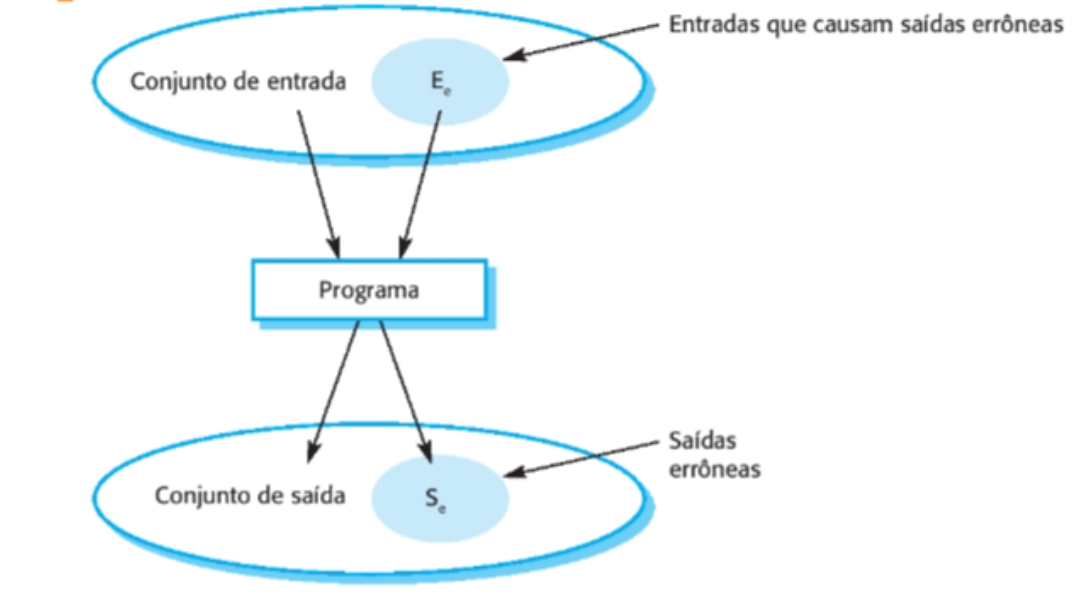
\includegraphics[width=0.9\linewidth]{entrada_saidas_erroneas.png}
    % \caption{falha}
\end{figure}
\end{frame}
\begin{frame}{Sistema como Mapeamento de Entradas/Saídas}
  \begin{figure}[h] % [h] tenta posicionar "aqui" (here)
    \centering % Centraliza a imagem
    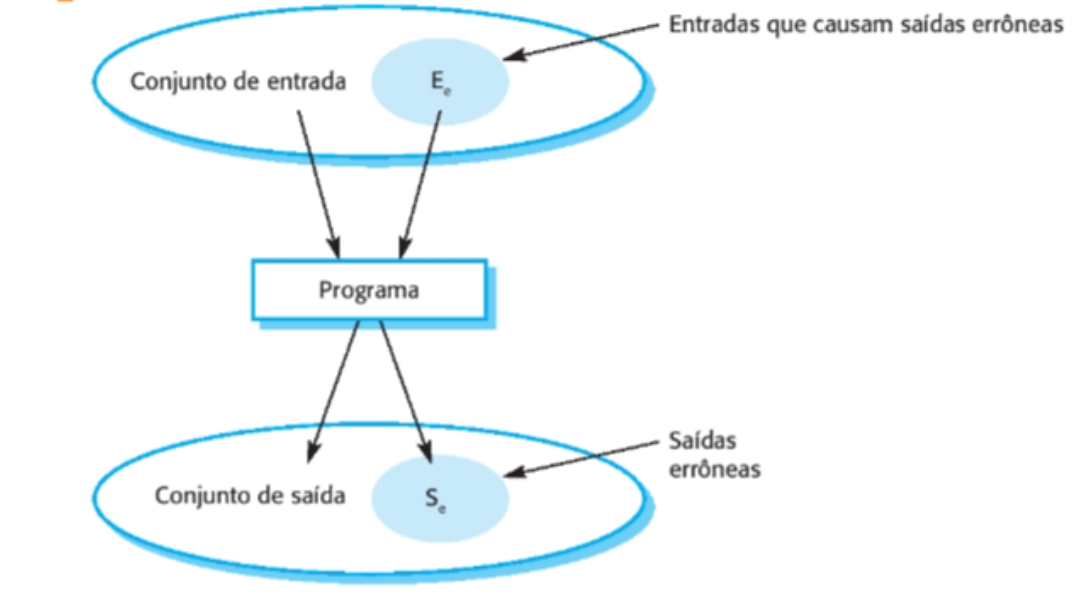
\includegraphics[width=0.7\linewidth]{entrada_saidas_erroneas.png}
    % \caption{falha}
\end{figure}
    \begin{exampleblock}{Exemplo Prático}
        Dada a entrada de uma URL, um navegador web produz a exibição da página solicitada como saída.
    \end{exampleblock}

    \begin{itemize}
        \item A maioria das entradas processadas não resulta em falhas.
        \item Entretanto, certas combinações de entradas ($E_e$) provocam falhas ou saídas errôneas.
    \end{itemize}
    
\end{frame}

% --- SLIDE: FREQUÊNCIA DE USO E FALHAS ---
\begin{frame}{O Impacto da Utilização na Confiabilidade}
    \begin{itemize}
        \item A confiabilidade depende de quantas entradas do conjunto $E_e$ são executadas no dia a dia.
        \item O conjunto $E_e$ representa as entradas que provocam a execução de código defeituoso e erros de sistema.
    \end{itemize}

    \begin{columns}[T]
        \begin{column}{0.5\textwidth}
            \begin{block}{Falhas Frequentes}
                Ocorrem se as entradas de $E_e$ fazem parte das funcionalidades mais utilizadas do sistema.
            \end{block}
        \end{column}
        \begin{column}{0.45\textwidth}
            \begin{block}{Falhas Raras}
                Ocorrem se as entradas de $E_e$ pertencem a códigos raramente acessados pelos usuários.
            \end{block}
        \end{column}
    \end{columns}
\end{frame}

% --- SLIDE: DIFERENTES PERCEPÇÕES ENTRE USUÁRIOS ---
\begin{frame}{Percepção de Confiabilidade por Usuário}
    \begin{itemize}
        \item Defeitos que afetam um usuário podem nunca aparecer no modo de trabalho de outro.
    \end{itemize}

    \begin{description}
        \item[Usuário 2:] Experimenta falhas, pois seu conjunto de entradas tem interseção com o conjunto errôneo $E_e$.
        \item[Usuários 1 e 3:] Nunca utilizam as entradas do conjunto errôneo.
    \end{description}

    \begin{figure}[h] % [h] tenta posicionar "aqui" (here)
    \centering % Centraliza a imagem
    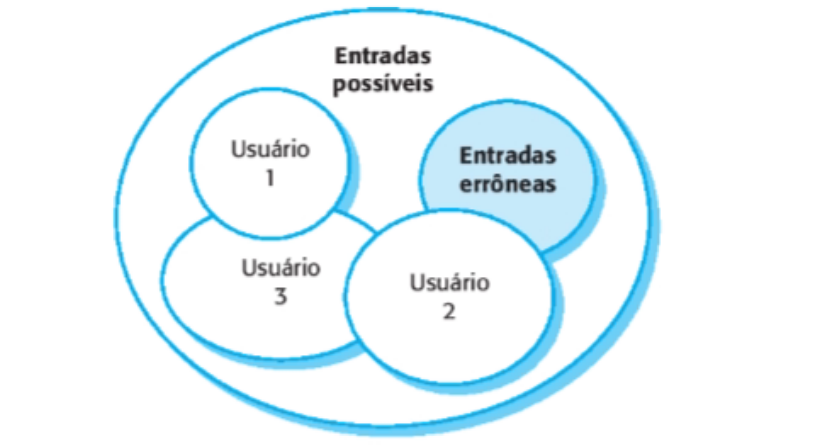
\includegraphics[width=0.6\linewidth]{padroes_usuarios.png}
    % \caption{falha}
\end{figure}

    \begin{alertblock}{Conclusão}
        Para os usuários 1 e 3, o software sempre parecerá 100\% confiável, mesmo que contenha defeitos.
    \end{alertblock}
\end{frame}
% --- SLIDE: DISPONIBILIDADE VS. FREQUÊNCIA DE FALHAS ---
\begin{frame}{Disponibilidade e Tempo de Reparo}
    \begin{itemize}
        \item A disponibilidade não depende apenas do número de falhas, mas também do \textbf{tempo necessário para consertar} os defeitos.
    \end{itemize}

    \begin{table}[]
        \small
        \begin{tabular}{|l|c|c|}
        \hline
        \textbf{Métrica} & \textbf{Sistema A} & \textbf{Sistema B} \\ \hline
        Frequência de Falha & 1 por ano & 1 por mês \\ \hline
        Tempo de Reinício & 6 horas (360 min) & 5 minutos \\ \hline
        \textbf{Parada Total/Ano} & \textbf{360 minutos} & \textbf{60 minutos} \\ \hline
        \end{tabular}
    \end{table}

    \begin{block}{Conclusão do Exemplo}
        Embora o Sistema A pareça mais confiável (falha menos), o \textbf{Sistema B tem uma disponibilidade muito maior} ao longo do ano.
    \end{block}
\end{frame}
\section{Impacto Real da Indisponibilidade}  

% --- SLIDE: O MOMENTO DA FALHA ---
\begin{frame}{Impacto Real da Indisponibilidade}
    \begin{itemize}
        \item A métrica de porcentagem simples de tempo disponível não reflete a \textbf{perturbação real} causada ao usuário.
        \item O \textbf{momento} em que a falha ocorre é um fator determinante.
    \end{itemize}

    \begin{columns}[T]
        \begin{column}{0.5\textwidth}
            \begin{exampleblock}{Cenário A: Baixo Impacto}
                Indisponibilidade de \textbf{1 hora} diária entre 3h00 e 4h00 da manhã. Afeta poucos usuários.
            \end{exampleblock}
        \end{column}
        \begin{column}{0.45\textwidth}
            \begin{alertblock}{Cenário B: Alto Impacto}
                Indisponibilidade de apenas \textbf{10 minutos} durante o horário comercial. Efeito muito maior nos usuários.
            \end{alertblock}
        \end{column}
    \end{columns}
\end{frame}

% --- SLIDE: CONFIABILIDADE VS. DISPONIBILIDADE ---
\begin{frame}{Prioridades em Sistemas Críticos}
    \begin{itemize}
        \item Confiabilidade e disponibilidade estão relacionadas, mas sua importância relativa varia conforme o uso.
    \end{itemize}

    \begin{description}
        \item[Alta Disponibilidade:] Requisito essencial quando os usuários esperam por um \textbf{serviço contínuo}. O sistema deve estar pronto sempre que houver demanda.
        \item[Recuperação Rápida:] Se o sistema se recupera de falhas sem perda de dados, o impacto percebido pelo usuário pode ser minimizado, mesmo com falhas frequentes.
    \end{description}

    \begin{center}
        \textit{"Uma falha rápida e segura pode ser preferível a uma falha rara, mas catastrófica."}
    \end{center}
\end{frame}
\section{Dependabilidade}  

% --- SLIDE: O QUE É DEPENDABILIDADE? ---
\begin{frame}{O Conceito de Dependabilidade}
    \begin{block}{Definição}
        É a propriedade de um sistema de computação que permite confiar justificadamente no serviço que ele entrega.
    \end{block}

    \textbf{Os Pilares da Dependabilidade:}
    \begin{columns}[T]
        \begin{column}{0.48\textwidth}
            \begin{itemize}
                \item \textbf{Disponibilidade:} Prontidão para o uso.
                \item \textbf{Confiabilidade:} Continuidade de serviço isento de falhas.
            \end{itemize}
        \end{column}
        \begin{column}{0.48\textwidth}
            \begin{itemize}
                \item \textbf{Segurança (Safety):} Ausência de consequências catastróficas.
                \item \textbf{Proteção (Security):} Resistência a intrusões e danos.
            \end{itemize}
        \end{column}
    \end{columns}

    \vspace{0.4cm}
    

    \begin{itemize}
        \item É uma \textbf{propriedade holística}: depende não apenas do software, mas também do hardware e das pessoas (operadores).
        \item Sistemas de alta dependabilidade são projetados para sobreviver a erros sem causar falhas.
    \end{itemize}
\end{frame}
% --- SLIDE: DEPENDABILIDADE E REQUISITOS ---
\begin{frame}{Dependabilidade: Além da Engenharia}
    \begin{itemize}
        \item A dependabilidade exige atenção minuciosa na \textbf{derivação} e no \textbf{ajuste} dos requisitos do sistema.
    \end{itemize}

    \begin{columns}[T]
        \begin{column}{0.5\textwidth}
            \begin{block}{1. Requisitos Funcionais}
                \small
                Definem recursos de:
                \begin{itemize}
                    \item Verificação e recuperação.
                    \item Proteção contra falhas e ataques externos.
                \end{itemize}
            \end{block}
        \end{column}
        \begin{column}{0.45\textwidth}
            \begin{block}{2. Requisitos Não Funcionais}
                \small
                Definem as metas de:
                \begin{itemize}
                    \item \textbf{Confiabilidade} necessária.
                    \item \textbf{Disponibilidade} necessária.
                \end{itemize}
            \end{block}
        \end{column}
    \end{columns}

    \begin{itemize}
        \item \textbf{Visão Holística:} A confiabilidade global depende do hardware, software e dos operadores.
        \item \textbf{Compensação de Erros:} O software deve incluir requisitos que ajudem na detecção e recuperação de falhas de hardware e erros humanos.
    \end{itemize}
\end{frame}
\section{Métricas de Confiabilidade}  

% --- SLIDE: MÉTRICAS DE CONFIABILIDADE (POFOD E ROCOF) ---
\begin{frame}{Métricas de Confiabilidade: POFOD e ROCOF}
    \begin{enumerate}
        \item \textbf{POFOD (Probabilidade de Falha Sob Demanda)}
        \begin{itemize}
            \item Probabilidade de uma requisição de serviço resultar em falha.
            \item \textbf{Exemplo:} $POFOD = 0,001$ indica 1 chance em 1.000 de falha ao acionar o sistema.
        \end{itemize}

        \vspace{0.3cm}
        \item \textbf{ROCOF (Taxa de Ocorrência de Falhas)}
        \begin{itemize}
            \item Número provável de falhas em um período de tempo ou execuções.
            \item \textbf{MTTF (Mean Time To Failure):} É o inverso da ROCOF ($1/ROCOF$).
            \item \textbf{Exemplo:} Se $ROCOF = 2$ falhas/hora, então $MTTF = 30$ minutos.
        \end{itemize}
    \end{enumerate}

    \begin{block}{Diferença Crucial}
        \small
        A POFOD é ideal para sistemas de proteção (ex: freio ABS), enquanto a ROCOF/MTTF é melhor para sistemas de uso contínuo (ex: servidores).
    \end{block}
    \begin{block}{MTTR - Mean Time To Repair}
    Representa a média do tempo gasto para realizar o reparo de falhas:
    \[ MTTR = \frac{T_{total\_manutencao}}{N_{reparos}} \]
    Quanto menor o valor, maior a \textbf{manutenibilidade} do sistema.
\end{block}
\end{frame}

\section{Métricas de Disponibilidade}
% --- SLIDE: DISPONIBILIDADE (AVAIL) ---
\begin{frame}{Disponibilidade (AVAIL)}
    \begin{itemize}
        \item Probabilidade de o sistema estar operacional no momento da demanda.
        \item Medida geralmente como uma porcentagem do tempo total de operação.
    \end{itemize}
    \begin{exampleblock}{Formula}
        $AVAIL = \frac{MTTF}{MTTF + MTTR}$ \\
      \end{exampleblock}
    \begin{table}[]
        \centering
        \small
        \caption{Impacto dos níveis de Disponibilidade em 24h}
        \begin{tabular}{|l|l|l|}
        \hline
        \textbf{AVAIL} & \textbf{Porcentagem} & \textbf{Tempo de Indisponibilidade} \\ \hline
        0,90           & 90\%                 & 144 minutos (2h 24min)             \\ \hline
        0,99           & 99\%                 & 14,4 minutos                       \\ \hline
        0,999          & 99,9\%               & 84 segundos                        \\ \hline
        0,9999         & 99,99\%              & 8,4 segundos                       \\ \hline
        \end{tabular}
    \end{table}

    \begin{itemize}
        \item \textbf{Os "Nove":} Na indústria, fala-se em "quatro noves" (99,99\%) para indicar sistemas de altíssima disponibilidade.
    \end{itemize}
\end{frame}

\section{Exercícios Resolvidos}
\begin{frame}{Exercício 1: POFOD}
    \begin{block}{Enunciado}
        Um sistema de acionamento de emergência de um gerador foi testado 500 vezes. Em 2 dessas ocasiões, o gerador não ligou quando solicitado. Qual é a \textbf{POFOD} deste sistema?
    \end{block}

    \pause
    \begin{exampleblock}{Resolução}
        $POFOD = \frac{\text{Número de Falhas}}{\text{Número de Demandas}}$ \\
        \vspace{0.2cm}
        $POFOD = \frac{2}{500} = 0,004$
    \end{exampleblock}

    \textbf{Resposta:} A probabilidade de falha sob demanda é de \textbf{0,4\%} (ou 4 falhas a cada 1.000 demandas).
\end{frame}\begin{frame}{Exercício 2: ROCOF e MTTF}
    \begin{block}{Enunciado}
        Um servidor web registrou 12 falhas durante um período de operação de 48 horas. Calcule a taxa de ocorrência de falhas (\textbf{ROCOF}) e o tempo médio até a falha (\textbf{MTTF}).
    \end{block}

    \pause
    \begin{exampleblock}{Resolução}
        $ROCOF = \frac{\text{Falhas}}{\text{Tempo}} = \frac{12}{48} = 0,25 \text{ falhas/hora}$ \\
        \vspace{0.3cm}
        $MTTF = \frac{1}{ROCOF} = \frac{1}{0,25} = 4 \text{ horas}$
    \end{exampleblock}

    \textbf{Resposta:} O sistema falha, em média, a cada \textbf{4 horas}.
\end{frame}\begin{frame}{Exercício 3: Disponibilidade Percetual}
    \begin{block}{Enunciado}
        Um sistema de banco de dados deve operar 24h por dia. Na última semana (7 dias), ele ficou fora do ar por um total de 70 minutos para manutenção emergencial. Qual foi a sua disponibilidade (\textbf{AVAIL})?
    \end{block}

    \pause
    \begin{exampleblock}{Resolução}
        Tempo total (min): $7 \times 24 \times 60 = 10.080 \text{ min}$ \\
        Tempo operacional: $10.080 - 70 = 10.010 \text{ min}$ \\
        \vspace{0.2cm}
        $AVAIL = \frac{10.010}{10.080} \approx 0,9930$
    \end{exampleblock}

    \textbf{Resposta:} A disponibilidade foi de aproximadamente \textbf{99,30\%}.
\end{frame}\begin{frame}{Exercício 3: Disponibilidade Percetual}
    \begin{block}{Enunciado}
        Um sistema de banco de dados deve operar 24h por dia. Na última semana (7 dias), ele ficou fora do ar por um total de 70 minutos para manutenção emergencial. Qual foi a sua disponibilidade (\textbf{AVAIL})?
    \end{block}

    \pause
    \begin{exampleblock}{Resolução}
        Tempo total (min): $7 \times 24 \times 60 = 10.080 \text{ min}$ \\
        Tempo operacional: $10.080 - 70 = 10.010 \text{ min}$ \\
        \vspace{0.2cm}
        $AVAIL = \frac{10.010}{10.080} \approx 0,9930$
    \end{exampleblock}

    \textbf{Resposta:} A disponibilidade foi de aproximadamente \textbf{99,30\%}.
\end{frame}\begin{frame}{Exercício 4: O Desafio dos "Três Noves"}
    \begin{block}{Enunciado}
        Se um cliente exige um contrato de nível de serviço (SLA) com disponibilidade de \textbf{0,999}, quanto tempo de parada (Downtime) é permitido em um mês comercial de 30 dias?
    \end{block}

    \pause
    \begin{exampleblock}{Resolução}
        Tempo total no mês: $30 \times 1.440 \text{ min} = 43.200 \text{ min}$ \\
        Indisponibilidade permitida: $1 - 0,999 = 0,001$ \\
        \vspace{0.2cm}
        $Downtime = 43.200 \times 0,001 = 43,2 \text{ minutos}$
    \end{exampleblock}

    \textbf{Resposta:} O sistema pode ficar fora do ar por no máximo \textbf{43,2 minutos} por mês.
\end{frame}\begin{frame}{Exercício 5: Confiabilidade vs. Disponibilidade}
    \begin{block}{Enunciado}
        O Sistema X tem $MTTF = 100h$ e leva $10h$ para reiniciar. O Sistema Y tem $MTTF = 20h$ e leva $1h$ para reiniciar. Qual deles tem a maior disponibilidade?
    \end{block}

    \pause
    \begin{exampleblock}{Resolução}
        $AVAIL = \frac{MTTF}{MTTF + MTTR}$ \\
        \vspace{0.2cm}
        $AVAIL(X) = \frac{100}{100+10} = \frac{100}{110} \approx \mathbf{0,909}$ \\
        $AVAIL(Y) = \frac{20}{20+1} = \frac{20}{21} \approx \mathbf{0,952}$
    \end{exampleblock}

    \textbf{Resposta:} O \textbf{Sistema Y} tem maior disponibilidade, apesar de falhar 5 vezes mais que o Sistema X.
\end{frame}
\end{document}
